% ---------------------------------------------------
% TSP 2016 Conference Template
% ---------------------------------------------------


\documentclass[conference,a4paper,twocolumn]{IEEEtran}

\IEEEoverridecommandlockouts


% *** GRAPHICS RELATED PACKAGES ***
%
\ifCLASSINFOpdf
\else
\fi


  \usepackage{tipa}
  \usepackage[pdftex]{graphicx}
	\usepackage{epsfig}
	\usepackage{epstopdf}


% *** MATH PACKAGES ***
%
\usepackage[cmex10]{amsmath}


% *** SUBFIGURE PACKAGES ***
\usepackage{subfigure}

\hyphenation{op-tical net-works semi-conduc-tor}

% *** CUSTOME (added by Alexander Senov) PACKAGES ***
%\usepackage[utf8x]{inputenc} % указывает кодировку документа
%\usepackage[T2A]{fontenc} % указывает внутреннюю кодировку TeX 
\usepackage[english]{babel} % указывает язык документа
%\usepackage{lmodern}
%\usepackage{gentium}
%\renewcommand*\rmdefault{phv}

\usepackage{graphicx}
\usepackage{subfig} % to make two figures side by side
%\usepackage{subcaption}
\usepackage{enumitem} % to specify enumeration start

\usepackage{color} % для цветного текста

\usepackage{lipsum} % for dummy text

\newcommand{\convnet}{ConvNet~} % я не знаю как правильно называть сетку в тексте, вместо этого вставляю эту команду

\newcommand{\todo}[1]{\textcolor{red}{\textbf{[#1]}}} % чтобы в глаза бросалось
% ---------------------------------------------------
% Begin of Document
% ---------------------------------------------------

\begin{document}

% ---------------------------------------------------
% Title
% ---------------------------------------------------

% Titles are generally capitalized except for words such as a, an, and, as,
% at, but, by, for, in, nor, of, on, or, the, to and up, which are usually
% not capitalized unless they are the first or last word of the title.
% Linebreaks \\ can be used within to get better formatting as desired.
% Do not put math or special symbols in the title.


\title{Arabic Manuscript Author Verification Using\\ 
Deep Convolutional Networks}

% ---------------------------------------------------
% Authors, Affiliation, and Acknowledgment
% ---------------------------------------------------



% conference papers do not typically use \thanks and this command
% is locked out in conference mode. If really needed, such as for
% the acknowledgment of grants, issue a \IEEEoverridecommandlockouts
% after \documentclass

% for over three affiliations, or if they all won't fit within the width
% of the page, use this alternative format:
% 
\author{
\IEEEauthorblockN{
Andrei Boiarov\IEEEauthorrefmark{1},
Alexander Senov\IEEEauthorrefmark{2},
Alexander Knysh\IEEEauthorrefmark{3} and
Dmitry Shalymov\IEEEauthorrefmark{4}
}
\IEEEauthorblockA{
	\IEEEauthorrefmark{1}\IEEEauthorrefmark{2}\IEEEauthorrefmark{4}
	Faculty of Mathematics and Mechanics\\
	Saint Petersburg State University\\
	Saint Petersburg, Russia\\
	Email: 
		\IEEEauthorrefmark{1}a.boiarov@spbu.ru, 
		\IEEEauthorrefmark{2}alexander.senov@gmail.com, 
		\IEEEauthorrefmark{4}dmitry.shalymov@gmail.com
}
\IEEEauthorblockA{
\IEEEauthorrefmark{3}Department of Near Eastern Studies\\
University of Michigan\\
St. Petersburg State University Laboratory of Analysis and Modeling of Social Processes\\
%Ann Arbor, Michigan 48104-1608, USA\\
Ann Arbor, Michigan, USA\\
Email: alknysh@umich.edu}
\thanks{This research is supported by Saint Petersburg State University grant 6.37.181.2014. The authors express their deep gratitude to Mrs. Evyn Kropf of the Hatcher Graduate Library who kindly facilitated access to the University of Michigan library resources.}
}

% use for special paper notices
%\IEEEspecialpapernotice{(Invited Paper)}




% make the title area
\maketitle


% ---------------------------------------------------
% Abstract
% ---------------------------------------------------

% As a general rule, do not put math, special symbols or citations
% in the abstract
\begin{abstract}
% \lipsum[5]
The problem of manuscript author verification is quite important nowadays and since manual verification has a subjectivity drawback, need in objective automatic methods arises. In this paper we propose an automatic method for author verification based on consecutive patches from image extraction and such a state of the art image classification algorithm as deep convolutional network with two types of patches extraction: connected components based and fixed-size sliding window based. We apply this method to specific problem of medieval Egyptian Arab historian al-Maqrizi's authorship verification of manuscript \textit{al-Khitat} which volume was recently discovered. Using appropriately collected ground-truth labelled data for convolutional network training purpose our method demonstrates very promising results on previously unseen manuscripts.


%The problem of manuscript author verification is quite important nowadays. Since manual verification has a subjectivity drawback, need in objective automatic methods arises. We propose an automatic method for author verification based on such foremost image classification method as deep convolutional network which encapsulate both features from image extraction and classification steps thus removing subjectivity even from features extraction step in contrast to most state of the art author verification methods. We apply the method to the problem of of recently discovered paper by questonable  al-Maqrizi's authorship verification for specific set of manuscripts images authored both by al-Maqrizi (positive class) and other authors (negative class). Using careful by-author train/validation/test set splitting, preprocessing and convolutional network training we achieve excellent classification accuracy on the test set. 

\end{abstract}

% no keywords

% For peer review papers, you can put extra information on the cover
% page as needed:
% \ifCLASSOPTIONpeerreview
% \begin{center} \bfseries EDICS Category: 3-BBND \end{center}
% \fi
%
% For peerreview papers, this IEEEtran command inserts a page break and
% creates the second title. It will be ignored for other modes.
\IEEEpeerreviewmaketitle

% ---------------------------------------------------
% Introduction
% ---------------------------------------------------

\section{Introduction}
\label{sec:introduction}
The present study was motivated by the recent discovery by Dr. Noah Gardiner of the holograph (autograph) copy of the third volume of al-Maqrizi's famous ``Description of Egypt'' in the Library of the University of Michigan (Michigan Islamic MS 605) \cite{Noah}. The full title of the manuscript is ``al-Mawa'iz wa-al-i'tibar fi dhikr al-khitat wa-al-athar'' (``The Book of Admonitions and Lessons in the Catalogue of Territorial Divisions and Historical Monuments''; usually cited simply as \textit{al-Khitat}). The manuscript was copied well after 818 A.H. (1415 C.E.) and was finished shortly after 831 (1427) by the celebrated Egyptian historian Taqi al-Din Ahmad Ibn 'Ali al-Maqrizi (d. 845/1442). It is the only known Maqrizi holograph (autograph) in the Americas. A number of elements in the codex, including the apparent age of the paper, lacunae in the text where the dates of certain events had not been filled in, and a number of marginal addenda and sewn-in inserts containing text found in the printed editions, led Dr. Gardiner to suspect that it might be a draft copy of the work. He visually collated the predominant hand of the codex and the inserts with some published images of al-Maqrizi's hand and felt that a match was highly likely. He then sent images of the codex to Prof. Frederic Bauden of the University of Liege, the author of numerous articles on al-Maqrizi autographs. Prof. Bauden confirmed that the codex was indeed copied by al-Maqrizi himself, and was thus a holograph (autograph). He identified it as the fair copy (the author's final version) of the third volume of al-Khitat, and thus the only fair copy of any volume of al-Khitat to have been found.

Given the importance of this discovery for the history of science (al-Maqrizi's \textit{al-Khitat} is one of the earliest descriptions of the topography of Cairo and ancient Egyptian monuments in its environs as well as Alexandria), a cross-disciplinary team of researchers affiliated with the St. Petersburg State University (Laboratory of Analysis and Modeling of Social Processes) decided to verify Dr. Gardiner's and Prof. Bauden's findings by using method based on deep convolutional networks.

Previously used methods for author verification of Arabic manuscript and for related fields were focused on developing of various types of features that can be obtained from a manuscript picture \cite{MBulacu}, \cite{DFecker}. In this paper we present a novel approach based on learning \todo{of or about?} deep hierarchical structure of features from the row image. This method belongs to the class of the deep learning algorithms \cite{DL} and uses convolutional network \cite{CNN} for feature extraction and prediction. Deep convolution networks since 2012 year \cite{Alexnet} became the state of the art in many areas of computer vision: objects recognition, face identification, optical character recognition, object detection, etc \cite{DL}.

The paper is organized as follows. In section~\ref{sec:the_data} a description of the data set used in experiments is given. Section~\ref{sec:the_method} contains presentation of our methodology of patches from image extraction, training deep convolution networks and making decision of manuscript author. In section~\ref{sec:results_and_description} we present the results of our experiments, whereupon we provide a conclusion.
%\pagebreak
	

\begin{figure*}[!t]
	\center
  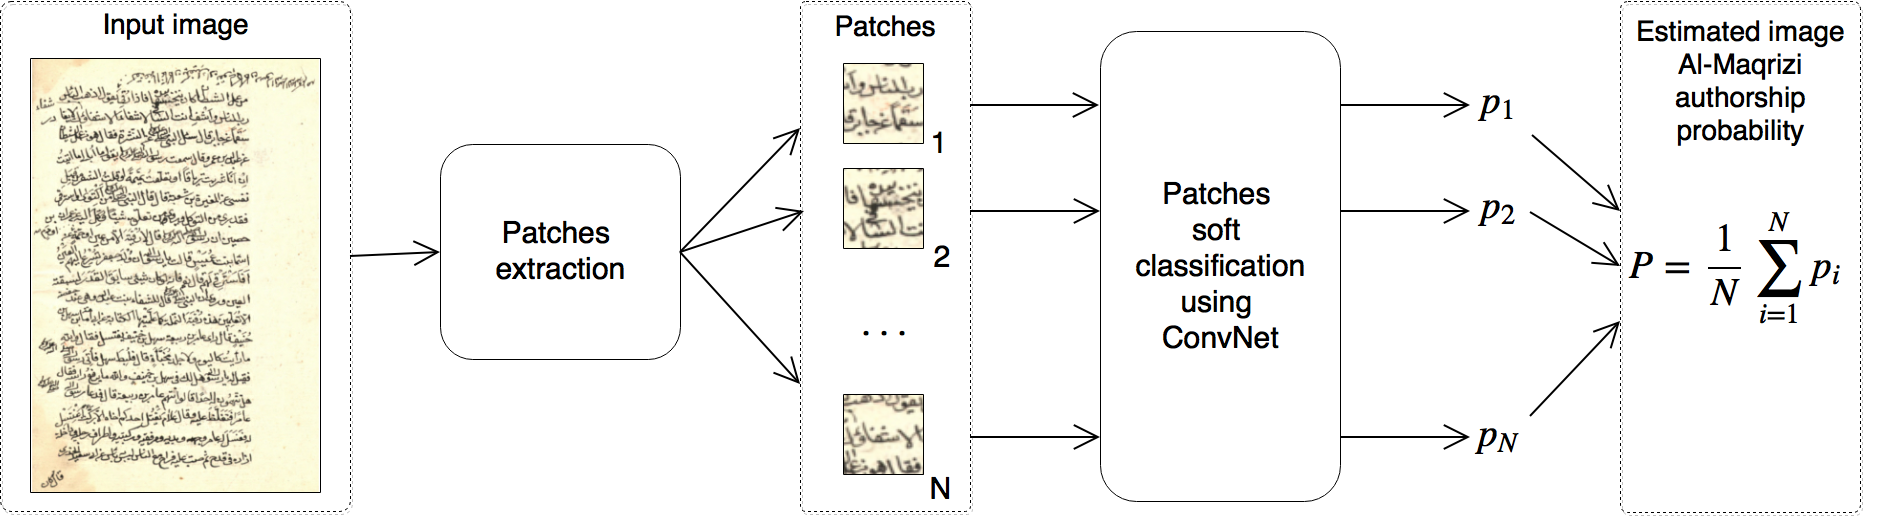
\includegraphics[width=0.9\textwidth]{figures/Al-Maqrizi_classification_pipeline.png}
  \caption{al-Maqrizi authorship classification pipeline}
  \label{fig:pipeline}
\end{figure*}	
	
\section{Data Set}
\label{sec:the_data}

Solving the problem of al-Maqrizi authorship verification requires training and test data sets. 
We consider a single page of the manuscript as one data unit.
As a one unique data element we consider single page of manuscript. The data set consists of two sets of manuscript materials:
\begin{itemize}
	\item two holographs of al-Maqrizi verified by Prof. Bauden will serve as a positive example;
	\item eight manuscripts not written by al-Maqrizi's hand  (taken from the University of Michigan Hatcher Library Special Collections) are considered to be a negative example. These manuscripts were selected in such a way that the date and place of writing of each of them would be close to those of al-Maqrizi's  \textit{al-Khitat}, namely, the 14th and 15th centuries, Egypt and Syria.
\end{itemize}

To enhance robustness of the learning process the data obtained were divided into training and test sets:
\begin{itemize}
	\item Training set: 1 al-Maqrizi's manuscript consisting of 26 pages and 5 not al-Maqrizi's manuscripts each of which consists of 7 pages.
	\item Test set: 1 al-Maqrizi's manuscript consisting of 14 pages and 3 non-al-Maqrizi's manuscripts each of which consists of 7 pages. Authors of these 3 manuscripts differ from authors of 5 negative examples in the training set.   
\end{itemize}

It is important to note that we split our data set by the factor of the manuscript author. When the algorithm is learning on the training set, it can not see the authors in the test set. Thus, we enforce our method to infer general properties al-Maqrizi's handwriting not specific for particular manuscript. Number of non-al-Maqrizi's documents is chosen in such way that positive and negative classes in training and test sets are roughly balanced.

The goal of this study is to verify the authorship of the \textit{al-Khitat} manuscript that consists of 32 pages. 


%\pagebreak

\section{Method}
\label{sec:the_method}

We consider author verification as a binary classification problem: al-Maqrizi class denoted as $1$ and non al-Maqrizi class denoted as $0$. In this context our goal is to build a classification pipeline able predict probability (\textit{soft} classification) that given image belongs to the $1$ (al-Maqrizi) class. The entire al-Maqrizi authorship classification pipeline illustrated at figure~\ref{fig:pipeline} consists of the following steps:

\begin{enumerate}[start=0]
	\item Image preprocessing.
	\item Extracting patches from candidate image.
	\item Patches soft classification using convolution network.
	\item Averaging predicted patches probabilities to produce overall candidate image al-Maqrizi authorship probability.
\end{enumerate}

Each of this steps are thoroughly described in the following sections.	

%The heart of our method is a \convnet patches classifier. We use ground-truth labelled patches extracted from images described in section~\ref{sec:the_data} as a training set for \convnet. [SOME DEFERRABLES FOR \convnet HERE].


\subsection{Image preprocessing}
This step was done to bring all images to relatively same size and scale by performing following steps:
\begin{enumerate}
	\item Removing part of image within the text bounding box.
	\item Resizing resulted image to resolution $700\times 500$.
\end{enumerate}
This steps are reasonable enough since all images from our data set has approximately equal number of text lines and text bounding box aspect ratio. 

Since this step is done only to unify our images data set we does not include it in the pipeline.

\subsection{Patches extraction}
The patches extraction method generates a set of sub-images called patches from given image. The basic idea is that patch should represent small but yet meaningful part of image for the main purpose --- authorship verification. We use two alternative methods for patches extraction described in following subsections.

\subsubsection{Sliding window based method}
This method splits image into patches by a grid of fixed cell of size $80\times 80$ pixels with a stride $20$ pixels. Figure~\ref{fig:patches_example_sliding_window} illustrates the idea. 

\subsubsection{Connected components based method}
This method uses following routine for patches extraction

\begin{enumerate}
	\item Input image binarization using Otsu's filter~\cite{otsu1975threshold}.
	\item Connected components extraction from binarized image using algorithm from~\cite{fiorio1996connected_components}.
	\item Too small, too big and too stretched connected components filtering using several empirical rules, e.g.: major axis to minor axis ratio less then $10$, minimum minor axis length greater then $3$ pixels, etc.
	\item Outlier connected components filtering using DBSCAN clustering algorithm~\cite{ester1996dbscan}, \cite{GranVolk}.
	\item Extracting remaining connected components bounding boxes from source image and resizing them $28\times 28$ pixels size.
\end{enumerate}

Example of connected components based patches show on figure~\ref{fig:patches_example_connected_components}. 

It can be seen, that connected components based patches usually consist of one or few letters thus providing high robustness for different image scale and size in contrast to fixed-size sliding window patches (since all images been preprocessed this features is not important in our case). However, sliding-window patches contain much more information: several symbols from multiple lines, --- a very important feature for the authorship verification.
%
%\begin{figure}[!b]
%    \centering
%    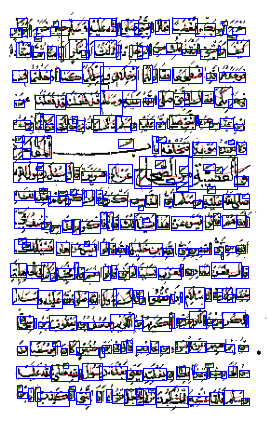
\includegraphics[width=0.2\textwidth]{figures/patches_example_connected_components.png}	 
%	\hfill    
%    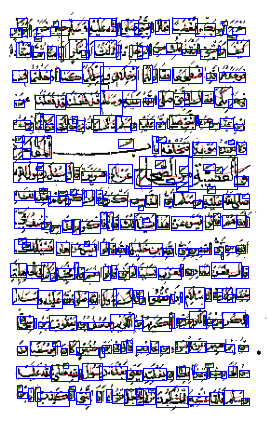
\includegraphics[width=0.2\textwidth]{figures/patches_example_connected_components.png} 
%%    \caption{2 Figures side by side}%
%    \label{fig:example}%
%\end{figure}

%\begin{figure}
%	\centering
%	\begin{minipage}{0.1\textwidth}
%	\centering
%	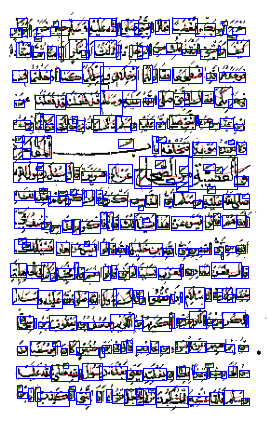
\includegraphics{figures/patches_example_connected_components.png}
%	\caption{first figure}
%	\end{minipage}
%	\hfill
%	\begin{minipage}{0.1\textwidth}
%	\centering
%	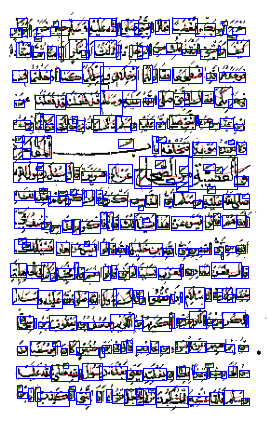
\includegraphics{figures/patches_example_connected_components.png}
%	\caption{second figure}
%	\end{minipage}
%\end{figure}

\begin{figure}
\centering
\begin{minipage}{.45\linewidth}
	\centering
  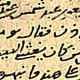
\includegraphics[height=.7\linewidth]{figures/3.png}
  \captionof{figure}{Sliding window patch example}
  \label{fig:patches_example_sliding_window}
\end{minipage}
\hspace{.05\linewidth}
\begin{minipage}{.45\linewidth}
	\centering
  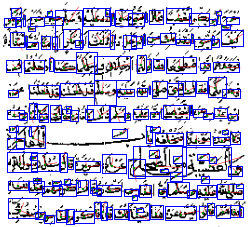
\includegraphics[height=.7\linewidth]{figures/patches_example_connected_components_part.png}
  \captionof{figure}{Connected components patches example}
  \label{fig:patches_example_connected_components}
\end{minipage}
\end{figure}

%\begin{figure}
%	\centering
%	\subcaptionbox{A cat\label{cat}}
%	[.4\linewidth]{\includegraphics{figures/patches_example_connected components.png}}%
%	\subcaptionbox{An elephant\label{elephant}}
%	[.4\linewidth]{\includegraphics{figures/patches_example_connected components.png}}
%	\caption{Two animals}\label{animals}
%\end{figure}

\subsection{Deep convolution network}

Denote $x_i$ as the $i$-th patch obtained from image in the previous step and $y_i$ as binary label. Then for predicting the probability
\begin{equation*}
	p_i = P(y_i | x_i)
\end{equation*}
that current patch belongs to al-Maqrizi's hand we need to train a discriminative model. As a robust and powerful classification algorithm deep convolution networks \cite{DL}, \cite{CNN} are chosen. 

In a case of sliding window patches we apply Alexnet type of network \cite{Alexnet}. Architecture of this network described in table~\ref{alexnet_tab}.
\begin{table}[!h]
\centering
\caption{Sliding window patch convolution network}
\label{alexnet_tab}
\begin{tabular}{|l|p{1.3cm}|p{1.3cm}|}
\hline
\textbf{type} & \textbf{patch size/ stride} & \textbf{output number}  \\
\hline
convolution & 11 / 4 & 96 \\
\hline
local response norm & & 96 \\
\hline
max pool & 3 / 2 & 96 \\
\hline
convolution & 5 / 1 & 256 \\
\hline
local response norm & & 256 \\
\hline
max pool & 3 / 2 & 256 \\
\hline
convolution & 3 / 1 & 384 \\
\hline
convolution & 3 / 1 & 384 \\
\hline
convolution & 3 / 1 & 256 \\
\hline
max pool & 3 / 2 & 256 \\
\hline
fully connected & & 4096 \\
\hline
dropout (50 \%) & & 4096 \\
\hline
fully connected & & 4096 \\
\hline
dropout (50 \%) & & 4096 \\
\hline
fully connected & & 2 \\
\hline
softmax & & 2 \\
\hline
\end{tabular}
\end{table}

As an input network takes $80\times80$ RGB image. All activation functions in convolution and fully connected layers is rectified linear units (ReLU). This deep network was trained by stochastic gradient descent method with Nesterov momentum, initial learning rate is $0.01$ and it decrease policy is step down.

With connected components patches we use GoogLeNet type of deep convolutional network \cite{Googlenet}. It architecture provided in table~\ref{googlenet_tab}. 
\begin{table}[!h]
\centering
\caption{Connected components patch convolution network}
\label{googlenet_tab}
\begin{tabular}{|l|p{1.3cm}|p{1.3cm}|}
\hline
\textbf{type} & \textbf{patch size/ stride} & \textbf{output number}  \\
\hline
convolution & 7 / 2 & 64 \\
\hline
max pool & 3 / 2 & 64 \\
\hline
local response norm & & 64 \\
\hline
convolution & 1 / 1 & 64 \\
\hline
convolution & 3 / 1 & 192 \\
\hline
local response norm & & 192 \\
\hline
max pool & 3 / 2 & 192 \\
\hline
inception &  & 256 \\
\hline
inception &  & 480 \\
\hline
max pool & 3 / 2 & 480 \\
\hline
inception &  & 512 \\
\hline
convolution & 1 / 1 & 128 \\
\hline
fully connected & & 1024 \\
\hline
dropout (70 \%) & & 1024 \\
\hline
fully connected & & 2 \\
\hline
softmax & & 2 \\
\hline
\end{tabular}
\end{table}

As an input network takes $28\times28$ RGB image. All activation functions in convolution and fully connected layers is rectified linear units (ReLU). Inception layer is a combination of several convolution and pooling layers, for more details see \cite{Googlenet}. Learning method for this convolutional network is stochastic gradient descent with Nesterov momentum and initial learning rate $0.01$ with step down decrease policy. 

\section{Results and Discussion}
\label{sec:results_and_description}

We experimented with both types of patches extraction and corresponding convolutional networks. 

\subsection{Deep convolutional network learning}

\begin{figure}[!ht]
\centering
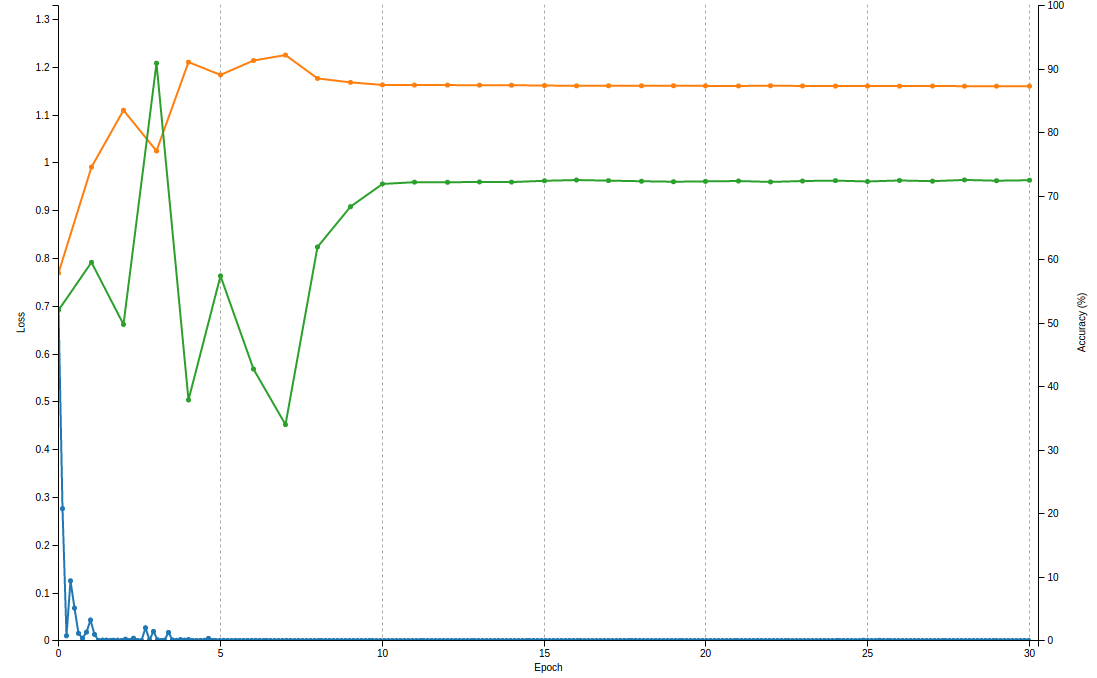
\includegraphics[scale=0.15]{figures/alexnet_loss.png}
\caption{Sliding window patch convolution network learning process.}
\label{img_alexnet}
\end{figure}

Figure~\ref{img_alexnet} demonstrates values of loss function on training (blue curve) and test (green curve) sets depending on the learning epoch for sliding window patch convolution network. Also one can see accuracy (orange curve) on the test set. It final value is near $87 \%$. For connected components patch convolution network accuracy is worse --- $80 \%$.    

\subsection{Manuscript classification}

To assess quality of the classification pipeline we use only images from the test set, since they are the only ones had not been used in the learning process. 

Figure~\ref{fig:al_maqrizi_classification_example} demonstrates classification result for two images from the test set: one from al-Maqrizi class and one from not al-Maqrizi class. As you can see, both of them classified quite confidently with estimated al-Maqrizi authorship probability $0.0085$ and $0.94$ respectively. Also this figure shows classification result for al-Khitat manuscript page. It gives $0.77$ probability of al-Maqrizi authorship.

\begin{figure}
\centering
\begin{minipage}{.48\linewidth}
	\centering
  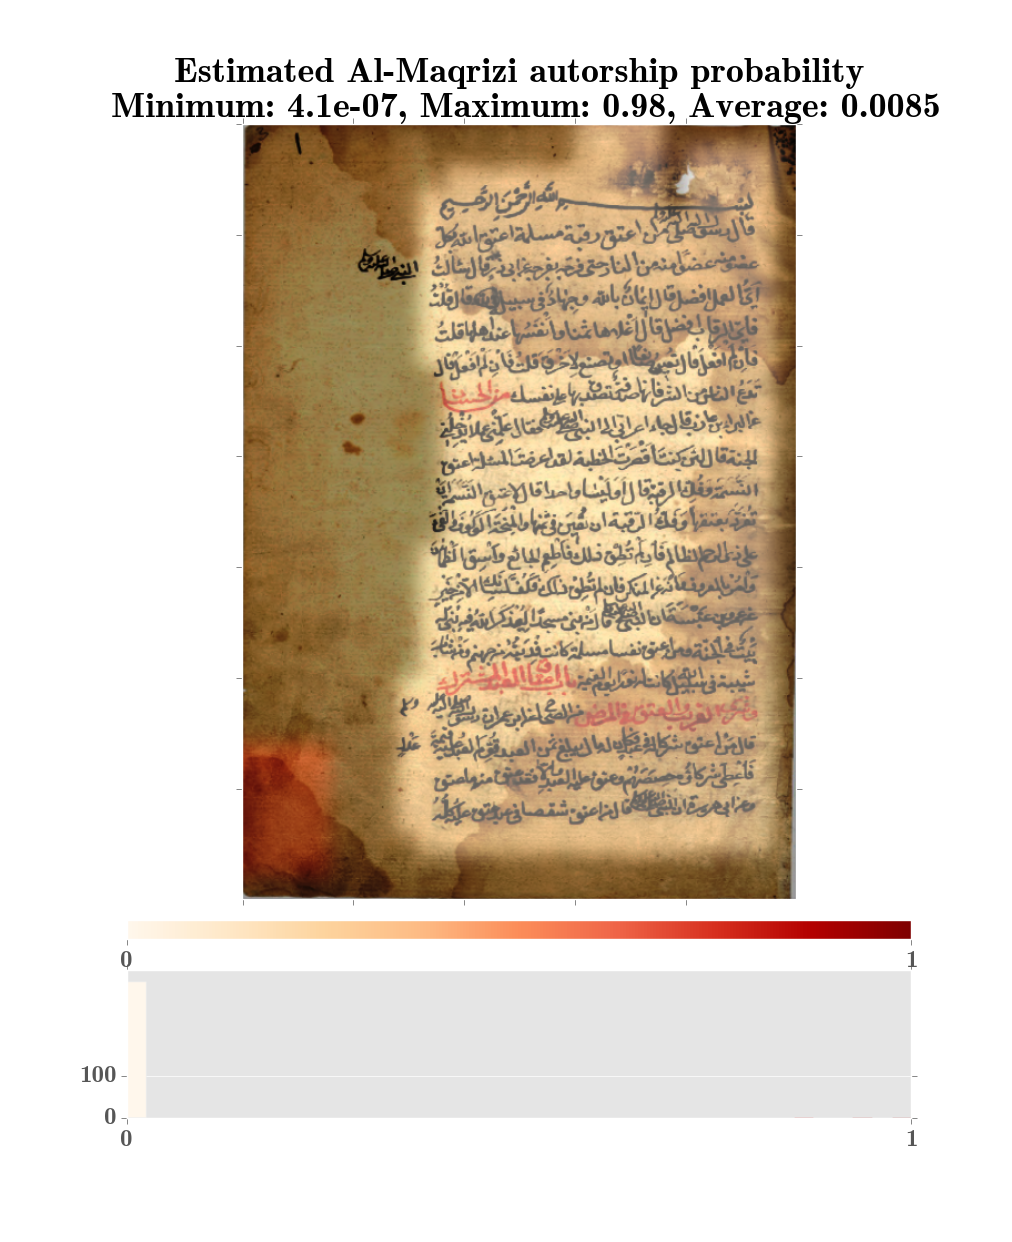
\includegraphics[width=\linewidth]{figures/not_al_maqrizi_image_classification_example.png}
  %\captionof{figure}{ }
  %\label{fig:}
\end{minipage}
\hspace{.01\linewidth}
\begin{minipage}{.48\linewidth}
	\centering
  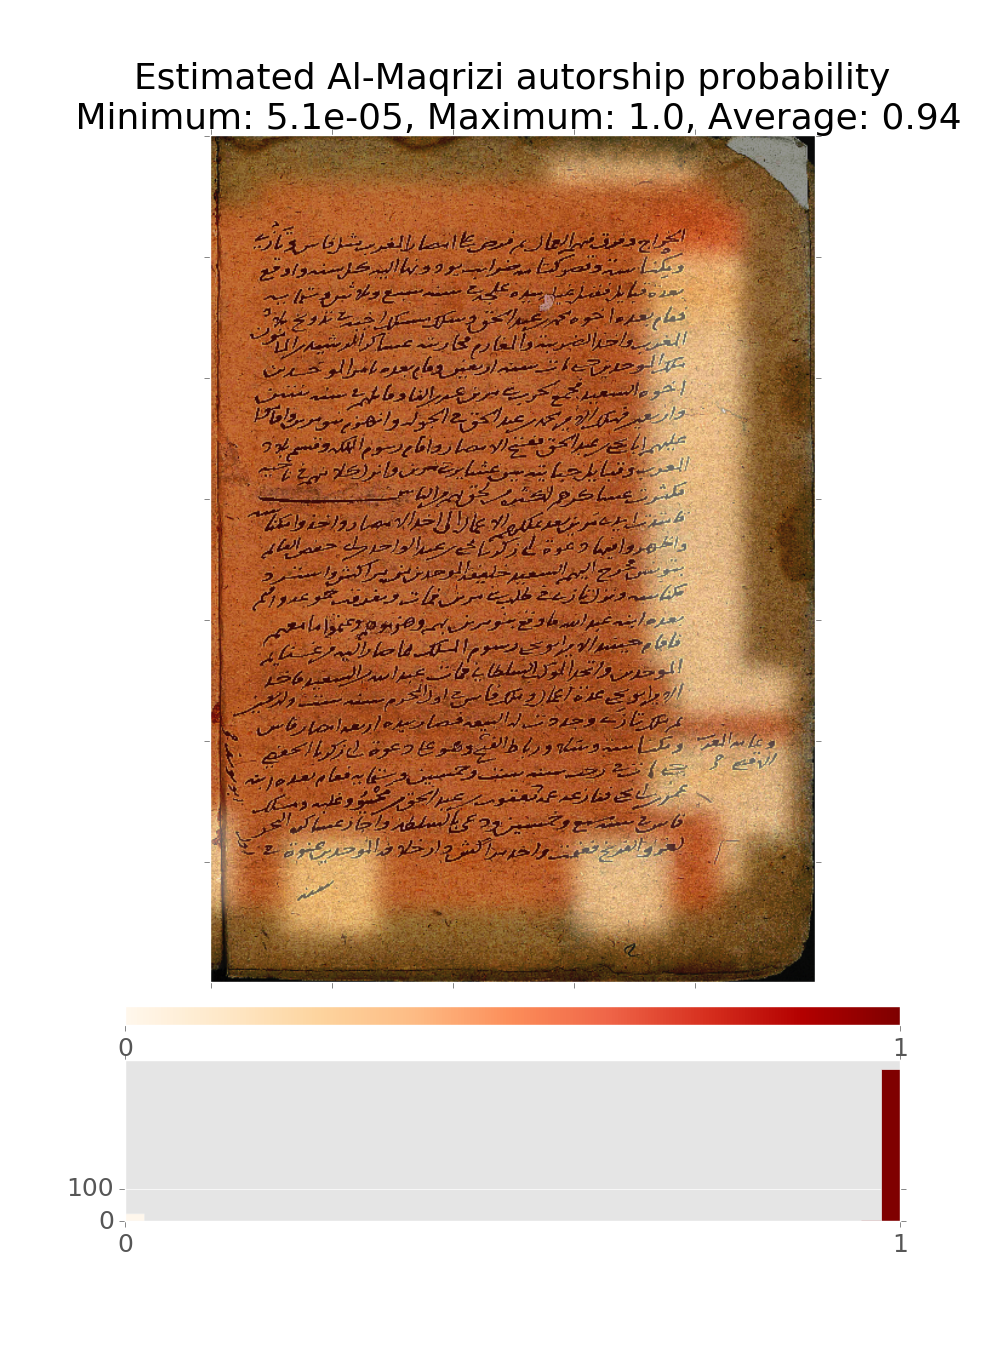
\includegraphics[width=\linewidth]{figures/sw_al_maqrisi.png}
  %\captionof{figure}{ }
  %\label{fig:}
\end{minipage}
\hspace{.01\linewidth}
\begin{minipage}{.48\linewidth}
	\centering
  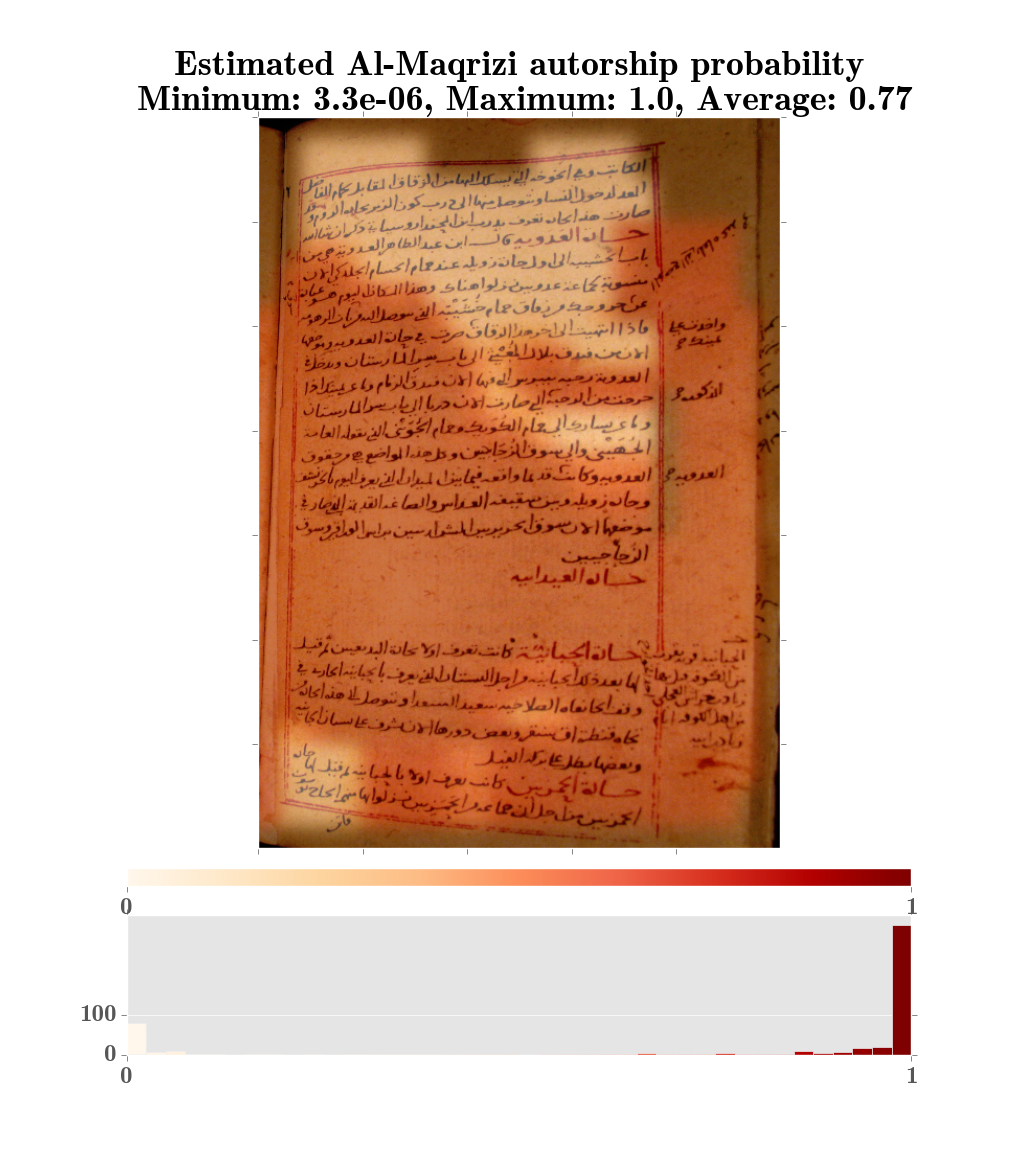
\includegraphics[width=\linewidth]{figures/hitat_15.png}
  %\captionof{figure}{ }
  %\label{fig:}
\end{minipage}
  \captionof{figure}{Sliding window patches al-Maqrizi authorship classification example: not al-Maqrizi manuscript page (left), al-Maqrizi manuscript page (right) and manuscript page from Khitat (bottom). Patches probabilities visualized using white-red colors (corresponding to 0-1 classes) on top of the original image. Additionally, probabilities histogram presented below.}
	\label{fig:al_maqrizi_classification_example}
\end{figure}

Regarding entire test set classification for sliding window patches with decision threshold $0.5$ we obtained precision $0.99$ and recall $0.92$. Method based on connected components patches is less robust: it generate many false positive predictions. But this approach has great potential and for it stable work required much more training examples. Thus convolutional network learned on connected components patches is prominent field for further research.

By using sliding window patches with deep network method we received that mean probability of al-Maqrizi authorship over all al-Khitat pages is equal to $0.86$.    

\section{Conclusion}

The join research on al-Maqrizi’s ``Description of Egypt'' undertaken by a historian-philologist and three mathematicians from St. Petersburg State University is a unique experiment in working across disciplinary boundaries to achieve a common goal. Its results bode well for the future by opening new horizons for scholars of ``Oriental'' manuscripts who often desperately lack resources (other than their own eyes and intuition) to verify the provenance and authorship of the manuscript material they are working with. Given the propensity of Muslim scribes and later writers to attribute manuscripts to important luminaries of the past (such as, e.g., al-Ghazali, d. 505/1111; Ibn al-Arabi, d. 638/1240, and others), the new methods of analyzing and verifying handwritten texts, which have been designed and tested by St. Petersburg mathematicians, are bound to become an important tool for their colleagues in the humanities and social sciences.

% ---------------------------------------------------
% References
% ---------------------------------------------------

% can use a bibliography generated by BibTeX as a .bbl file
% BibTeX documentation can be easily obtained at:
% http://www.ctan.org/tex-archive/biblio/bibtex/contrib/doc/
% The IEEEtran BibTeX style support page is at:
% http://www.michaelshell.org/tex/ieeetran/bibtex/
%\bibliographystyle{IEEEtran}
% argument is your BibTeX string definitions and bibliography database(s)
%\bibliography{IEEEabrv,../bib/paper}
%
% <OR> manually copy in the resultant .bbl file
% set second argument of \begin to the number of references
% (used to reserve space for the reference number labels box)

\begin{thebibliography}{99}

\bibitem{Noah} N.~Gardiner, F.~Bauden, \lq\lq A Recently Discovered Holograph Fair Copy of al-Maqrizi's al-Mawa'iz wa-al-i'tibar fi dhikr al-khitat wa-al-athar (Michigan Islamic MS 605),\rq\rq~in~\emph{Journal of Islamic Manuscripts}, vol.~2, E.~J.~Brill, Leiden and Boston, 2011, pp.~123--131.

\bibitem{MBulacu} M.~Bulacu, L.~Schomaker, A.~Brink \lq\lq Text-independent writer identification and verification on offline arabic handwriting,\rq\rq~in~\emph{Proc. 9th International Conference on Document Analysis and Recognition, ICDAR}, Curitiba, 2007, pp.~769--773.

\bibitem{DFecker} D.~Fecker, A.~Asi, W.~Pantke, V.~Märgner, J.~El-Sana, T.~Fingscheidt \lq\lq Document Writer Analysis with Rejection for Historical Arabic Manuscripts,\rq\rq~in~\emph{Proc. 14th nternational Conference on Frontiers in Handwriting Recognition, ICFHR}, Crete, 2014, pp.~743--748.

\bibitem{DL} Y.~Lecun, Y.~Bengio, G.~Hinton, \lq\lq Deep learning,\rq\rq~\emph{Nature}, no.~521, pp.~436--444, May.~2015.

\bibitem{CNN} Y.~Lecun, L.~Bottou, Y.~Bengio, P.~Haffner, \lq\lq Gradient-based learning applied to document recognition,\rq\rq~in~\emph{Proc. of the IEEE}, 1998, pp.~2278--2324.

\bibitem{Alexnet} A.~Krizhevsky,I.~Sutskever, G.~Hinton, \lq\lq ImageNet Classification with Deep Convolutional Neural Networks,\rq\rq~in~\emph{Advances in Neural Information Processing Systems}, vol.~25, 2012, pp.~1097--1105.

\bibitem{Googlenet} C.~Szegedy, W.~Liu, Y.~Jia, P.~Sermanet, S.~Reed, D.~Anguelov, D.~Erhan, V.~Vanhoucke, A.~Rabinovich, \lq\lq Going deeper with convolutions,\rq\rq~in~\emph{Proc. of the IEEE Conference on Computer Vision and Pattern Recognition}, Boston, 2015, pp.~1--9.

\bibitem{otsu1975threshold} N.~Otsu, \lq\lq A threshold selection method from gray-level histograms, \rq\rq~\emph{Automatica}, vol.~11, 1975, pp.~285--296.

\bibitem{fiorio1996connected_components} C.~Fiorio, J.~Gustedt, \lq\lq Two linear time union-find strategies for image processing, \rq\rq~\emph{Theoretical Computer Science}, vol.~154, no.~2, 1996, pp.~165--181.

\bibitem{ester1996dbscan} M.~Ester, H.P.~Kriegel, J.~Sander, X.~Xu, \lq\lq A density-based algorithm for discovering clusters in large spatial databases with noise, \rq\rq~in~\emph{Proc. of Second International
Conference on Knowledge Discovery and Data Mining}, vol.~96, no.~34, 1996, pp.~226--231.

\bibitem{GranVolk} O.~Granichin, V.~Volkovich, D.~Toledano-Kitai, \emph{Randomized Algorithms in Automatic Control and Data Mining}. Springer-Verlag: Heidelberg, New York, Dordrecht, London, 2015, 251~p.

\end{thebibliography}

% ---------------------------------------------------
% End of Document
% ---------------------------------------------------

% that's all folks
\end{document}


